% siminos/blog/atlas.tex
% $Author$ $Date$

\chapter{Atlas}
\label{chap:atlas}

\begin{description}
\item[2011-11-30 Predrag]
started a new blog, for Predrag's putative letter

\texttt{siminos/atlas/main.tex}

\item[2011-12-06 Roman] However,  ECS can be used to project
trajectories onto a low-dimensional visualization where coordinates $a^k_{i}(t)$
are defined by the inner product
\beq
\label{coordinatesRG}
a^k_{i}(t)= \frac{1}{V} \int_V {\bf e}^k_i(t)^\dagger\cdot({\bf u}(t)-{\bf u}^k(t)) dV,
\eeq
%\pagebreak
where $V$ is the flow domain volume, ${\bf u}^k(t)$ is the ECS closest to
the system state at time $t$, and ${\bf e}^k_i(t)$ are basis functions
representing a set of unstable and weakly stable modes characterizing the
particular ECS.

\item[2011-12-06 Predrag]
Mhm - why are we introducing new notation for \statesp\
coordinates in \refeq{coordinatesRG}? I cannot imagine a situation in which one
would like to make the bases  ${\bf e}^k_i$ time dependent, ${\bf e}^k_i(t)$,
and we mostly use ECS themselves to construct projections, as in
\reffig{f:ssptransient}, not their stability eigenvectors. If you are really
thinking of using ECS's ${\bf u}^k(t)$ as templates whose linearized local
charts compose a global atlas for the flow, they would not be time dependent,
but fixed by a set of Poincar\'e sections to \statesp\ points ${\bf u}^k$, and
the associated set of unstable and weakly stable eigenvectors (what are
"modes"?) ${\bf e}_i^k$ would also be confined to the Poincar\'e section, and
not time dependent. But I think this is way too sophisticated for referees to
wrap their heads around....

I propose you drop time dependence from ${\bf e}^k_i(t)$ and ${\bf
u}^k(t)$ and pass over all that in silence for now. Or perhaps keep the
formula as is, as neither the authors themselves have never sorted out
how the \po\ eigenvectors are to be used in practice.

\begin{figure}
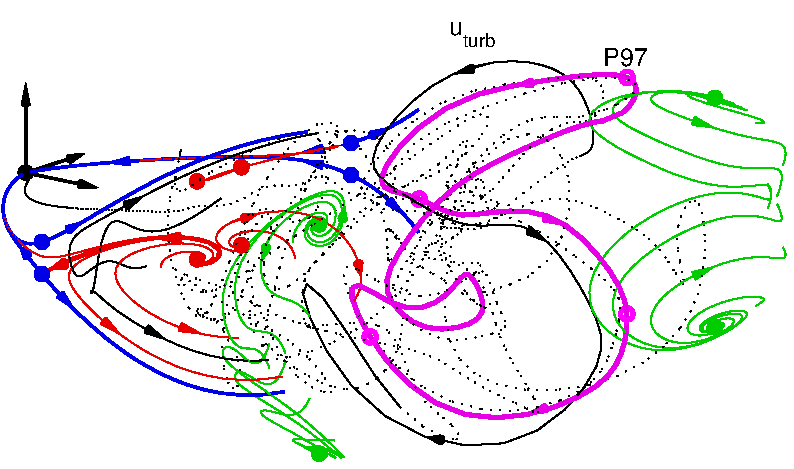
\includegraphics[width=\textwidth]{P97portrait5}
\caption{
{\bf A state-space portrait of turbulent plane Couette flow.}
A turbulent trajectory ${\bf u}_{\text{turb}}$ (solid and dotted black
lines) shadowing the P97 periodic orbit (bold magenta line) and the
unstable manifolds (blue, red, and green lines) of symmetry-related
equilibria (solid blue, red, and green dots; the black dot at the origin
is the laminar flow state). Velocity fields corresponding to the open
magenta dots on P97 are shown in  reffig~{f:ssptransient2}. Dynamic
connections are shown as bold red and blue lines connecting different
equilibria (filled dots).
}
\label{f:ssptransient}
\end{figure}

\item[2011-12-06 John] Predrag's comment on \refeq{coordinatesRG} is on
target: it makes sense with the verbal description attached to it, but
the time-dependence of the basis set $e_i^k(t)$ and the nearest ECS
$u^k(t)$ is pretty confusing. The bigger problem is that the equation as
is reflects what we want to do, but doesn't the projection in
\reffig{f:ssptransient}, which uses a fixed basis based on four
symmetry-related ECS to produce a global portrait.

\item[2012-02-18 Predrag] clippings

This procedure has been devised by Poincar\'e in the context of celestial
mechanics, in the aim of reducing the analysis of long-term planetary
motion and its dynamic stability [Poincar\'e, Les m\'ethodes nouvelles de
la m\'ecanique c\'eleste 1892].

\begin{figure}
  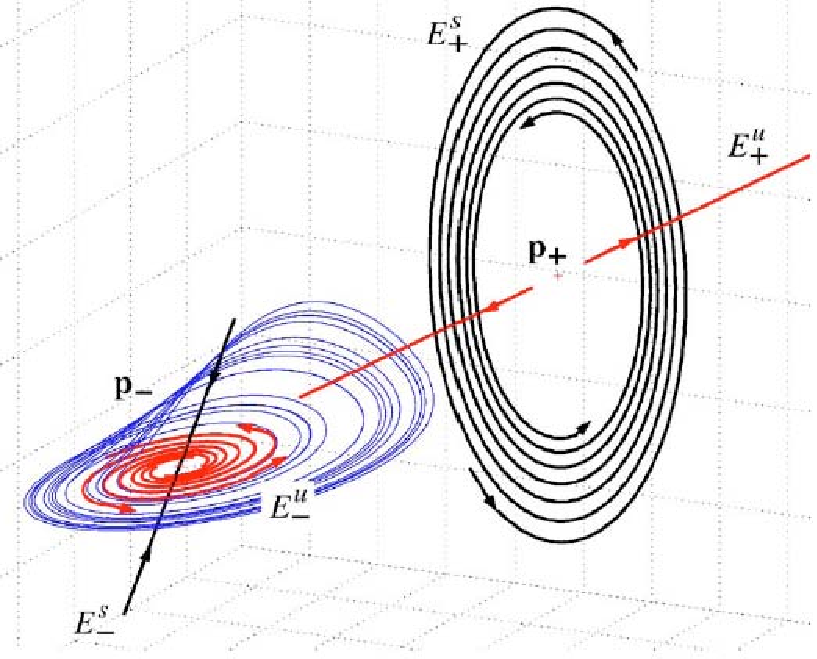
\includegraphics[width=0.6\textwidth]{AmLeAg06Im1}\\
  \caption{From \refref{AmLeAg06}:
R\"ossler attractor with fixed points and their manifolds. The linear
stable manifold at the lower fixed point is 1-dimensional and the
unstable one is associated with an unstable focus. The stable manifold at
upper fixed point is a stable focus and the unstable manifold is
1-dimensional}
\label{fig:AmLeAg06Im1}
\end{figure}

From \refref{AmLeAg06}:
``A linear system is $\dot{x} =Ax$ and an affine system is $\dot{x}
=Ax+b$, where $A$ is a constant matrix and $b$ is a constant vector.''

                                            \toCB
Draw (un)stable eigenvectors as in \reffig{fig:AmLeAg06Im1}.
``
In the R\"ossler system, the switching is induced by the
nonlinearity which acts when the trajectory is sufficiently far
from lower fixed point, that is, beyond the threshold $x-c$ in
the third equation. The nonlinearity
acts when the trajectory is sufficiently close to upper fixed
points where its converging spiral induces the folding by
sending the trajectory back to the neighborhood of lower fixed
point along its unstable manifold. Thus, the lower fixed point
is mainly responsible for the stretching and upper fixed point for
the folding.
''

\end{description}
